\section{Subgradient Methods}

  \begin{definition}[Convex Function]
    A function $f: U \subset \mathbb{R}^n \rightarrow \mathbb{R}$ defined on a convex set $U$ is convex if and only if for any $\mathbf{x}, \mathbf{y} \in U$
    \begin{equation}
      f \big(\lambda \mathbf{x} + (1 - \lambda) \mathbf{y} \big) \leq \lambda f(\mathbf{x}) + (1 - \lambda) f(\mathbf{y})
    \end{equation}
    Now if $f$ is differentiable, then convexity is equivalent to 
    \begin{equation}
      f(x) \geq f(y) + \nabla f(y)^T \cdot (x - y)
    \end{equation}
    for all $x, y \in U$. That is, its local linear approximation always underestimates $f$. 
  \end{definition}

  It is well known that the mean square error of a linear map is convex. However, when we impose the L1 penalty, the loss function is now not differentiable at $\mathbf{0}$. Therefore, we must introduce the notion of a subgradient. 

  \begin{definition}[Subgradient]
    The subgradient of a convex function $f: U \subset \mathbb{R}^n \rightarrow \mathbb{R}$ is any linear map $\mathbf{A} (x): \mathbb{R}^n \rightarrow \mathbb{R}$ such that 
    \begin{equation}
      f(\mathbf{y}) \geq f(\mathbf{x}) + \mathbf{A}(\mathbf{x}) (\mathbf{y} - \mathbf{x})
    \end{equation}
    for any $\mathbf{y} \in U$. The set of all subgradients at $\mathbf{x}$ is called the \textbf{subdifferential} defined 
    \begin{equation}
      \partial f (\mathbf{x}) = \{ \mathbf{A} \in \mathbb{R}^n \mid \mathbf{A} \text{ is a subgradient of } f \text{ at } \mathbf{x} \}
    \end{equation}
  \end{definition}

  The subgradient also acts as a linear approximation of $f$, but now at nondifferentiable points of convex functions, we have a set of linear approximations. It is clear that the subgradient at a differentiable point is uniquely the gradient ($\partial f(\mathbf{x}) = \{ \nabla f(\mathbf{x})$), but for places like the absolute value, we can have infinite linear approximations. 
  \begin{center}
    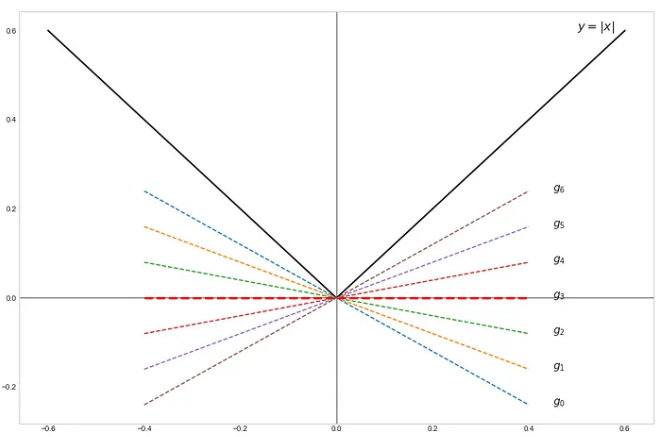
\includegraphics[scale=0.4]{img/subgradient_of_abs.png}
  \end{center}
  Given the subdifferential, thus the optimality condition for any convex $\mathbf{f}$ (differentiable or not) is
  \begin{equation}
    f(\mathbf{x}^\ast) = \min_{\mathbf{x}} f(\mathbf{x}) \iff \mathbf{0} \in \partial f(\mathbf{x}^\ast)
  \end{equation}
  known as the subgradient optimality condition, which clearly implies 
  \begin{equation}
    f(\mathbf{y}) \geq f(\mathbf{x}^\ast) + \mathbf{0}^T (\mathbf{y} - \mathbf{x}^\ast) = f(\mathbf{x}^\ast)
  \end{equation}

  \begin{example}
    The subdifferential of the absolute value function $f(x) = |x|$ at any given $x$ is 
    \begin{equation}
      \partial f(x) = \begin{cases} 1 & \text{ if } x > 0 \\ [-1, 1] & \text{ if } x = 0 \\ -1 & \text{ if } x < 0 \end{cases}
    \end{equation}
  \end{example}

\subsection{Proximal Gradient Descent}

  \begin{definition}[Proximal Operator]
    Given a lower semicontinuous convex function $f$ mapping from Hilbert space $X$ to $[-\infty, +\infty]$, its \textbf{proximal operator} associated with a point $u$ is defined 
    \begin{equation}
      \prox_{f, \tau} (u) = \argmin_{x} \bigg( f(x) + \frac{1}{2\tau} ||x - u||^2 \bigg)
    \end{equation}
    where $\tau > 0$ is a parameter that scales the quadratic term. This is basically the point that minimizes the sum of $f(x)$ and the square of the Euclidean distance between $x$ and $u$, scaled by $1/2\tau$. 
  \end{definition}

  Now given the loss function $L (\boldsymbol{\theta}) = L_{\mathrm{obj}} (\boldsymbol{\theta}) + L_{\mathrm{reg}} (\boldsymbol{\theta})$, we want to compute the proximal operator on the regularization loss and update that with the gradient of the smooth objective loss. 
  \begin{equation}
    \boldsymbol{\theta}^{(k+1)} = \prox_{L_{\mathrm{reg}}, \tau} \big[ \boldsymbol{\theta}^{(k)} - \tau \nabla L_{\mathrm{obj}} (\boldsymbol{\theta}^{(k)}) \big]
  \end{equation}
  Let's compute the proximal operator of the L1 loss $h(\boldsymbol{\theta}) = \lambda ||\boldsymbol{\theta}||_1$. We can parameterize this loss by the $\lambda$, so we will use the notation $\prox_{\lambda, \tau}$ rather than $\prox_{h, \tau}$. 
  \begin{align*}
    \prox_{\lambda, \tau} (\mathbf{u}) & = \argmin_{\boldsymbol{\theta}} \bigg( \lambda ||\boldsymbol{\theta}||_1 + \frac{1}{2\tau} ||\boldsymbol{\theta} - \mathbf{u}||_2^2 \bigg) \\
    & = \argmin_{\boldsymbol{\theta}} \bigg( \sum_{i=1}^n \lambda |\theta_i| + \frac{1}{2\tau} (\theta_i - u_i)^2 \bigg) 
  \end{align*}
  These are separable functions that can be decoupled and optimized component-wise. So, we really just want to find 
  \begin{equation}
    \theta_i^\ast = \argmin_{\theta_i} \bigg( \lambda |\theta_i| + \frac{1}{2\tau} (\theta_i - u_i)^2 \bigg)
  \end{equation}
  The sum of convex functions is convex, and so we should differentiate it and find where the gradient is $0$ to optimize it. 
  \begin{enumerate}
    \item When $\theta_i > 0$, then we minimize $\lambda \theta_i + \frac{1}{2\tau} (\theta_i - u_i)^2$, so taking the gradient and setting to $0$ gives 
    \begin{equation}
      \theta_i = u_i - \lambda \tau
    \end{equation}
    subject to the constraint that $\theta_i > 0$, or equivalently, that $u_i > \lambda \tau$. 

    \item When $\theta_i < 0$, then we minimize $-\lambda \theta_i + \frac{1}{2\tau} ( \theta_i - u_i)^2$, so taking the gradient and setting to $0$ gives 
    \begin{equation}
      \theta_i = u_i + \lambda \tau
    \end{equation}
    subject to the constraint that $\theta_i < 0$, or equivalently, that $u_i < -\lambda \tau$. 

    \item When $\theta_i = 0$, then we minimize $\lambda |\theta_i| + \frac{1}{2\tau} (\theta_i - u_i)^2$, which doesn't have derivative at $\theta_i = 0$. So, we can compute the subdifferential of it to get 
    \[0 \in \partial \bigg( \lambda |\theta_i| + \frac{1}{2\tau} (\theta_i - u_i)^2 \bigg) = \lambda \partial (|\theta_i|) + \frac{1}{\tau} (\theta_i - u_i)\]
    Now at $\theta_i = 0$, the subdifferential can be any value in $[-1, 1]$, and the above reduces to 
    \begin{equation}
      0 \in \lambda [-1, 1] - \frac{1}{\tau} u_i
    \end{equation}
    this is equivalent to saying that $u_i/\tau$ is contained in the interval $[-\lambda, \lambda]$, meaning that $u_i \in [-\lambda \tau, \lambda \tau]$. 
  \end{enumerate}

  Ultimately we get that 
  \begin{equation}
    \prox_{\lambda, \tau} (u) = \begin{cases} u - \lambda \tau & \text{ if } u > \lambda \tau \\ 0 & \text{ if } |u| \leq \lambda \tau \\ u + \lambda \tau & \text{ if } u < - \lambda \tau \end{cases}
  \end{equation}
  which can be simplified to 
  \begin{equation}
    \prox_{\lambda, \tau} (u) = \mathrm{sign}(u) \max\{ |u| - \lambda \tau, 0)
  \end{equation}

